\documentclass[11pt]{article}
\usepackage{geometry}                % See geometry.pdf to learn the layout options. There are lots.
\geometry{letterpaper}                   % ... or a4paper or a5paper or ... 
%\geometry{landscape}                % Activate for for rotated page geometry
%\usepackage[parfill]{parskip}    % Activate to begin paragraphs with an empty line rather than an indent
\usepackage{graphicx}
\usepackage{amssymb}
\usepackage{epstopdf}
% Package for including code in the document
\usepackage{listings}

\usepackage{algorithm,algorithmic}
\DeclareGraphicsRule{.tif}{png}{.png}{`convert #1 `dirname #1`/`basename #1 .tif`.png}

\title{Preliminary Report on MDA work}
\author{Dan Beatty}
%\date{}                                           % Activate to display a given date or no date

\begin{document}
\maketitle
%\section{}
%\subsection{}

The first part of the assignment was 
\begin{quote}
	You are given a total of 150 four dimensional samples of three Iris species.  Use Multiple Discriminant Analysis (MDA) to separate the samples into three Iris species. Show the resulting misclassifications.   Repeat MDA choosing any three-dimensional features at a time and show the resulting misclassifications.
\end{quote}

The Mathematica version is long mostly from listing the samples.  Other than that, the steps mimic the algorithm for MDA very closely.  Once the structure allows for a classifier to is constructed on the assumption that the data is Gaussian.  

\begin{lstlisting}{language=Mathematica}
barSetosa = Mean[setosa]
barSetosaArray = PadLeft[{barSetosa}, First[Dimensions[setosa]], {barSetosa}]
normSetosa = setosa - barSetosaArray
ScatterSetosa = Transpose[normSetosa].normSetosa/First[Dimensions[setosa]]

barVersicolor = Mean[versicolor]
barVersicolorArray = PadLeft[{barVersicolor}, First[Dimensions[
  versicolor]], {barVersicolor}]

normVersicolor = versicolor - barVersicolorArray
ScatterVeriscolor =
         Transpose[normVersicolor].normVersicolor/First[Dimensions[versicolor]\
]

barVirginica = Mean[virginica]
barVirginicaArray = PadLeft[{barVirginica}, First[Dimensions[virginica]], \
{barVirginica}]
normVirginica = virginica - barVirginicaArray
ScatterVirginica = \
Transpose[normVirginica].normVirginica/First[Dimensions[virginica]]
whiteningScatter = ScatterVirginica + ScatterSetosa + ScatterVeriscolor
flowers = Join[setosa, versicolor, virginica]
combinedMean = Mean[flowers]
flowers = Join[setosa, versicolor, virginica]
combinedMean = Mean[flowers]
meanArray = Join[{barSetosa}, {barVersicolor}, {barVirginica}]
combineMeanArray = PadLeft[{combinedMean}, Dimensions[meanArray], \
{combinedMean}]
meanDifference = (meanArray - combineMeanArray)
scatterBackground = Transpose[meanDifference] .(50*meanDifference)
{lambda, W} = Eigensystem [{scatterBackground, whiteningScatter}, 2]
ListPlot[flowers.Transpose[W]]
\end{lstlisting}

\subsection{Explanation of the Mathematica Code}
In the Mathematica example, we use setosa, viriginica, and versicolor as variables containing the original measurements.  We next construct an row matrix contain at each of its rows, called barSetosaArray.  This array is used to generate $\vec{x_i} - \mu$ for row vector $\vec{x_i}$ in the setosa collection, misnomered as normSetosa.  This allows mean to generate the scatter matrix for setosa.  

The same thing was done for versicolor and virginica.  As stated in the MDA algorithm, $\mathbf{S_w}=  \sum_i S_i$ where $S_i$ are the scatter matrices for each of the classes.  Here also, we combine the flowers using the Join method in Mathematic, and take a mean of the combined whole.  From there, we use the mean array concept to reduce finding the background scatter to matrix addition, scalar multiplication, matrix multiplication and a transpose.  

Fortunately, Mathematica has an intuitive method for computing eigenvectors of a generalized system as below.
\[
\mathbf{A} \vec{e_i} = \lambda_i \mathbf{B} \vec{e_i}
\]
Thus mapping the original data source via the $\mathbf{W}$ obtained is simply a matter of matrix multiplication

\subsection{Plot Results from Mathematica}
\begin{figure}[htbp] %  figure placement: here, top, bottom, or page
   \centering
   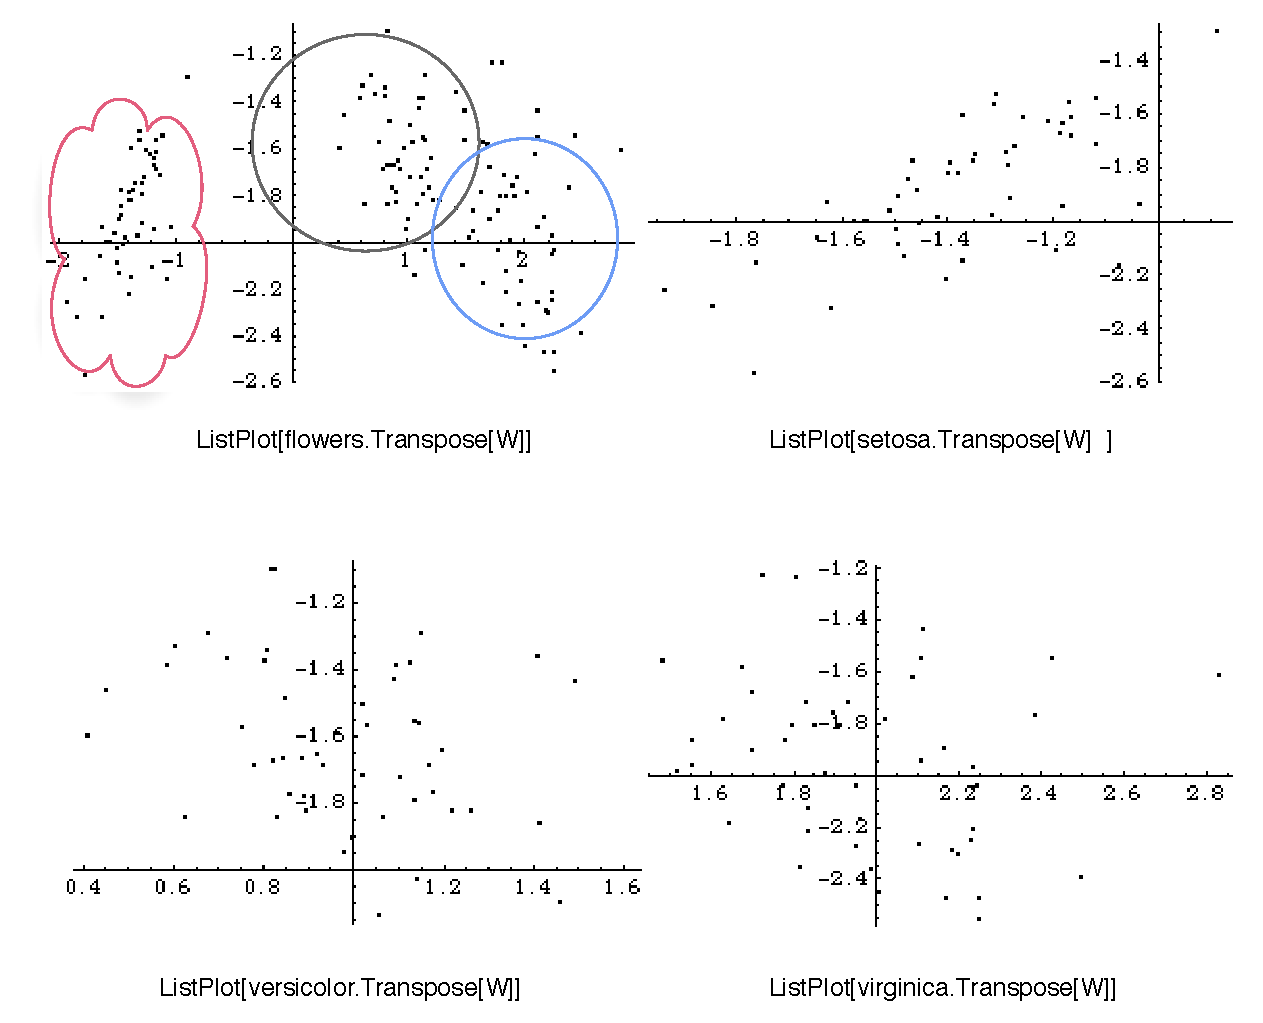
\includegraphics[width=5in]{flowersMDA.pdf} 
   \caption{mathematica Plots using a manual MDA}
   \label{mathematicaPlotsUsingManualMDA}
\end{figure}


\section{Objective-C Version of the MDA Classifier}
In order to satisfy the Multiple Discriminant Analysis (MDA) section of the problem, this solution has taken on two forms.  One, a solution in Mathematica, solve the preconditioner by hand and shows demonstration of concept.  The other is an automated library to be service that can be used in general.  Lessons from the Mathematica demonstration provides means for the unit tests of the object class.  For the sake of this discussion data class shall refer set for classifying the data into.  Object class shall refer to the Objective-C structure used to construct objects. 

The classic definition of Multiple Discriminant Analysis is defined by Algorithm \ref{alg:multiple_discriminant_analysis}.  In this definition, $D_i$ are the data classes, $\vec{m_i}$ are the sample mean of these data classes, $n_i$ are the number of samples in these data classes, $\vec{m_t}$ is the total mean for the samples of all of the data classes, and 

\begin{algorithm}
\caption{Multiple Discriminant Analysis}
\label{alg:multiple_discriminant_analysis}
\begin{algorithmic}
	\STATE Determine $\vec{m_t}$
	\FORALL{Classes $D_i$ in Discriminant Set $D$}
		\STATE Compute $\vec{m_i}$
		\STATE Determine $n_i$
		\STATE Determine $\hat{m_i} = \vec{m_i} - \vec{m_t}$
		\STATE Compute $S_i = \sum_{\vec{x_i} \in D_i} (\vec{x_i} - \vec{m_i} )(\vec{x_i} - \vec{m_i} )^T $
	\ENDFOR
	\STATE $S_w = \sum _{S_i \in D} S_i$
	\STATE Compute $S_B = \sum_{\hat{m_i} \in D} n_i \hat{m_i}$
	\STATE Compute Top eigenvectors for equation: 
	\[
	\mathbf{S_B} \mathbf{w_i} = \lambda_i \mathbf{S_W} \mathbf{w_i}
	\]
	\RETURN {$\mathbf{W}, \mathbf{\Lambda} $}
\end{algorithmic}
\end{algorithm}


The MDA is all about conditioning the data to one less component than there is a data class.  The components are usually arranged as the columns of a matrix, $\mathbf{W}$.  If the original data is arranged as row vectors in a matrix $\mathbf{X}$, then
\begin{equation}
\mathbf{XW} = \mathbf{Y}
\end{equation}
where $\mathbf{Y}$ is a matrix the same number of rows, $m$, as sample matrix and $c-1$ columns where $c$ are the number of data classes.  Each of the columns are mappings onto an ortho-normal basis.  

The Objective-C version has two constructors.  One takes an array of ``sample classes'' which are simply structures containing the original samples, the mean, covariance, and scatter matrix.  The other takes a matrix containing the samples and a vector containing a enumerated mapping of row vector to class.    In the second, the ``sample classes'' are constructed so that the preconditioning matrix $W$ may be computed.  The preconditioning matrix $W$ is defining feature of the object class, and should be the thing requested from the structure.  

In order to construct the preconditioning matrix, there are two sets of methods based on data classes (sample classes) to generate the matrices required.  These two matrices are the background scatter matrix ($\mathbf{S_b}$) and whitening scatter matrix ($\mathbf{S_w}$).  

Compute Whitening Scatter is derived on the basis that a data class structure produces a scatter matrix on initialization.  Thus computing whitening scatter matrix is merely an addition of all of the scatter matrices.  

\begin{equation}
\mathbf{S_w} = \sum _i \mathbf{S_i}
\end{equation}

In order to construct the background scatter matrix, one needs a few supplemental matrices.  Most mathematical definitions of MDA do not state this explicitly, yet it is a necessary step for efficiency.  

The computation for the scatter matrices used to construct the pre-conditioner is as follows:
\begin{itemize}
	\item Number of Samples Vector $\vec{n}$
	\item Number of Samples Matrix $\mathbf{N}$
	\item Mean Transformation Matrix $\mathbf{M}$
\end{itemize}
The background scatter matrix is defined from these structures as:
\begin{equation}
	\mathbf{S_b} = (\mathbf{N} \cdot \mathbf{M})(\mathbf{M}^T) 
\end{equation}
where the cdot indicates a dot-Multiply between $\mathbf{N}$ and $\mathbf{M}$.  %This method allows the classic definition of the background scatter matrix to be performed as a consequence 

Real trick is how the eigenvectors are computed for $S_w$ and $S_b$. In this case, it is convenient to note the characteristic equation being solved.
\begin{eqnarray}
\mathbf{S_B}\vec{e_i} = \lambda_i \mathbf{S_w}\vec{e_i} \label{character_mda}\\
\mathbf{S_w}^{-1}\mathbf{S_B}\vec{e_i} = \lambda_i \mathbf{S_w}^{-1} \mathbf{S_w}\vec{e_i} \\
\mathbf{S_w}^{-1}\mathbf{S_B}\vec{e_i} = \lambda_i \mathbf{I} \vec{e_i} \\
\mathbf{S_w}^{-1}\mathbf{S_B}\vec{e_i} = \lambda_i \vec{e_i} \label{character-mda-singlematrix}
\end{eqnarray}
Most would argue that solving equation \ref{character_mda} would be the proper choice.  However, the Objective-C version does not have such a method.  It can compute inverses of square matrices, and eigenvectors of the characteristic equation \ref{eigenvector-character} which is the same as equation \ref{character-mda-singlematrix}.
\begin{equation}
\mathbf{A} \vec{e_i} = \lambda_i \vec{e_i} \label{eigenvector-character}
\end{equation}


\section {Plotting Libraries}
One library necessary for plotting these results come from the CGContext and CGContextArcToPoint.  These are presented in Laden and Gelphman chapter 5 and page 57.  

\end{document}  